\chapter{Introduction}

This board allows to connect FPix modules using a flex cable to connect it to the DTB. Its key features are:
\begin{itemize}
    \item Make the proper electrical connections between the TBM of the module and the DTB. This includes matching the impedances.
    \item Provide pass-through for the supply voltages.
    \item Provide a resistor bridge for measuring the temperature of the HDI using its RTD and two ADC channels in the DTB.
    \item Has an 2\,kbit EEPOM to identify the type of adapter, connected to the DTB via its \isqc{} bus.
\end{itemize}

The following conventions are used throughout this document:
\begin{itemize}
    \item SCSI-connector: this refers to the 68-pin connector, which will be used to connect the adapter to the DTB.
    \item SMK-connector: this is a 2$\times$20 pin connector to connect to the FPix module using standard FPix flex cables.
    \item GND: ground.
    \item HV: High voltage, routed through the DTB and supplied by an external power supply.
    \item VA: Supply voltage for analog circuits in the ROC.
    \item VD: Supply voltage for digital circuits in the TBM and ROC.
    \item 3V3: 3.3\,V supply for support circuits.
    \item TBM: Token bit manager, custom ASIC on the HDI
    \item HDI: High-density interconnect, custom circuit on modules, makes connections between TBM and ROC
    \item ROC: Read-out chip
    \item DTB: Digital test board
\end{itemize}
This document is not a full documentation of the whole chain. Please refer to the specific documents about other parts.

\chapter{Design considerations}
The board has been designed as a 4-layer PCB with the following topology:
\begin{center}
\begin{tabular}{cc}
	\toprule %-------------------------------------------------------------------------------------------------
Layer & Description \\
	\midrule %-------------------------------------------------------------------------------------------------
Top & Main signal layer \\
2nd & GND plane \\
3rd & Power plane, distributed $VA$, $VD$, and $HV$
	\bottomrule %-------------------------------------------------------------------------------------------------
\end{tabular}
\end{center}

\section{Signal routing}

The signal connections between the TBM and the DTB are as follows:
\begin{center}
\begin{tabular}{llll}
    \toprule %-------------------------------------------------------------------------------------------------
    TBM & direction & DTB & Comments \\
    \midrule %-------------------------------------------------------------------------------------------------
    \texttt{OutA}        & $\rightarrow$ & \texttt{SDATA1} & \\
    \texttt{RDa\_Out}    & $\rightarrow$ & \texttt{TOUT}   & \\
    \texttt{SD\_In}      & $\leftarrow$  & \texttt{SDA}    & \\
    \texttt{Trig\_In}    & $\leftarrow$  & \texttt{CTR}    & \\
    \texttt{Clk\_In}     & $\leftarrow$  & \texttt{CLK}    & \\
    \texttt{RClk\_Out}   & $\rightarrow$ & \texttt{SDATA3} & Not for regular use. Some TBM versions may not provide it. \\
    \texttt{160MHz\_Out} & $\rightarrow$ & \texttt{SDATA4} & Not for regular use. Some TBM versions may not provide it. \\
    \bottomrule %-------------------------------------------------------------------------------------------------
\end{tabular}
\end{center}


\section{Impedance matching of TBM signals}

The impedances of the two outer connections are not the same:
\begin{center}
\begin{tabular}{lc}
    \toprule %-------------------------------------------------------------------------------------------------
    Connection & Impedance $Z$ \\
    \midrule %-------------------------------------------------------------------------------------------------
    SCSI 68 pin & 115\,$\Omega$ \\
    SMK flex cable & 60\,$\Omega$ \\
    \bottomrule %-------------------------------------------------------------------------------------------------
\end{tabular}
\end{center}

The impedance matching is done following a proposal by Beat Meier of PSI and is sketched out in Fig.~\ref{fig:mpedmatch}. The values calculated are:
\begin{center}
\begin{tabular}{lc}
    \toprule %-------------------------------------------------------------------------------------------------
    Resistor & value \\
    \midrule %-------------------------------------------------------------------------------------------------
    $R_1$ & 39\,$\Omega$ \\
    $R_2$ & 91\,$\Omega$ \\
    \bottomrule %-------------------------------------------------------------------------------------------------
\end{tabular}
\end{center}
This choice of resistors are available in the E24 series and lead to the following differential impedances:
\begin{equation}
Z_1 = 2R_1 + \frac{1}{1/R_2 + 1/Z_2} = 115\,\Omega
\end{equation}
and
\begin{equation}
Z_2 = \frac{1}{\frac{1}{2R_1+Z_1}+\frac{1}{R_2}} = 62\,\Omega
\end{equation}
which is well within a few \% of the target impedances.

The dimensions of the traces on the board were caluclated using the PCBcalc app provided by Agilent. The values have been chosen as:
\begin{center}
\begin{tabular}{lcc}
    \toprule %-------------------------------------------------------------------------------------------------
    Parameter & Case 115\,$\Omega$ & Case 60\,$\Omega$ \\
    \midrule %-------------------------------------------------------------------------------------------------
    Dielectric constant $\epsilon_r$ & \multicolumn{2}{c}{4.20 (FR-4)} \\
    $h$ & \multicolumn{2}{c}{11.90\,mil (0.30\,mm)} \\
    $t$ & \multicolumn{2}{c}{1.70\,mil (0.043\,mm)} \\
    $w$ & 8.2\,mil (0.21\,mm) & 27\,mil (0.68\,mm) \\
    $s$ & 7.0\,mil (0.18\,mm) & 7.0\,mil (0.18\,mm) \\
    \bottomrule %-------------------------------------------------------------------------------------------------
\end{tabular}
\end{center}
The given values $\epsilon_r$, $h$ and $t$ were taken from the supplier (Sunstone circuits). The other values were chosen on practical reasons, where $w$ has been chosen to be a bit larger than the smallest distance the supplier recommends.


\begin{figure}[hbtp]
	\begin{center}
	\includegraphics[width=.3\textwidth]{img/impedmatch.pdf}
	\end{center}
	\caption{Impedance matching network. Assuming $Z_1>Z_2$, this network adjusts for properly chosen $R_1$ and $R_2$ the imedances according to requirements. The line thickness on the PCB board indicate proper matching there as well.}
	\label{fig:mpedmatch}
\end{figure}

\begin{figure}[hbtp]
	\begin{center}
	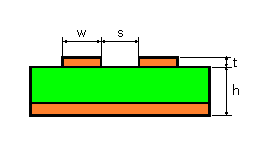
\includegraphics[width=.3\textwidth]{img/diffpair.pdf}
	\end{center}
	\caption{Sketch to define sme characteristic sizes in a differential pair trace on a PCB with a potential surface below the insulator.}
	\label{fig:diffpair}
\end{figure}


\section{RTD bridge}
Current versions of the HDI have a Pt10000 RTD for measuring the temperature. A circuit proposed by M. Matulik is shown in Fig.~\ref{fig:RTDcircuit}. This circuit is included and hooked up to two ADC channels of the DTB available on the SCSI connector.

\begin{figure}[hbtp]
	\begin{center}
	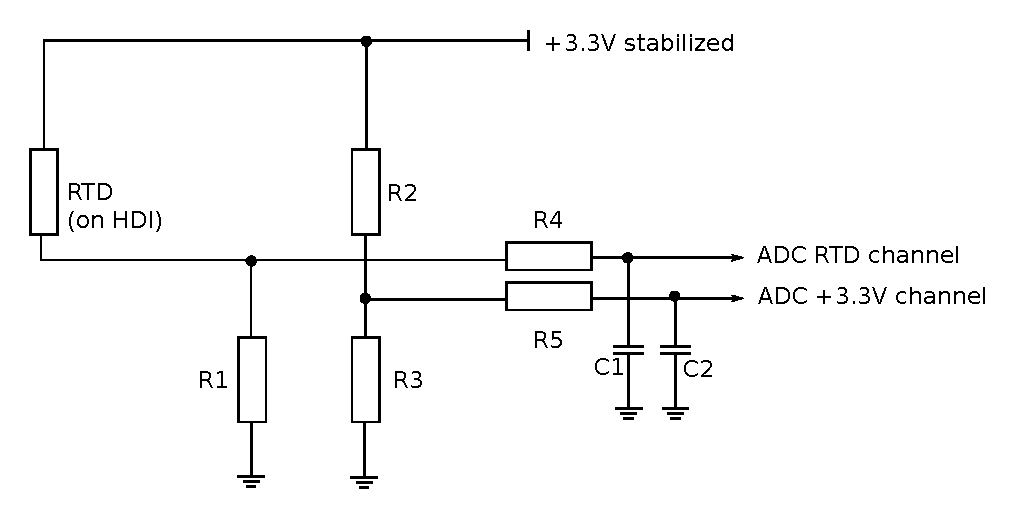
\includegraphics[width=.3\textwidth]{img/RTDcircuit.pdf}
	\end{center}
	\caption{RTD circuit. Two ADC channels are used for measuring the voltage of the RTD and 3.3\,V channel. The latter is used as a reference. The resolution is estimated to be 2\,$\circ$C.}
	\label{fig:RTDcircuit}
\end{figure}


\section{Form factor}

The size of the board are driven by the following requirements:
\begin{itemize}
    \item The PSI coldbox takes up to four modules, spaced by 6\,cm. The flex cables will therefore com out of the cold volume in the same spacing (center to center).
    \item The SCSI connectors come 
\end{itemize}

\section{HV protection}
High voltage is supplied via the DTB\footnote{The DTB has a relay to control HV from a HV power supply and passes it via a 100\,k$\Omega$ resistor to the SCSI cable. See the DTB documentation about its HV safety.}. The following measures have been taken:
\begin{itemize}
    \item The HV is routed entirely in an inner layer.
    \item There are some spots on the board where a HV is exposed:
    \begin{enumerate}
	\item HV pin at the SCSI connector (pin 68). Accessible on the back of the board.
	\item Two vias around the SMK connector
    \end{enumerate}
\end{itemize}

